\chapter{Conexión}%
\label{cha:conexion}
En este capítulo vamos a estudiar cuándo podemos decir que un conjunto está ``conectado'', o dicho de otro modo, cuando no está dividido en trozos y qué significa esto. Además, al final vamos a estudiar cómo se comporta esta nueva propiedad con respecto a las construcciones que hemos estudiado.

\section{Concepto y mantras}%
\label{sec:concepto_y_mantras_conx}
El concepto fundamental de conexión es que no estás dividido en trozos y precisamente esta es la idea intuitiva de la definición formal que viene a continuación. En esta sección vamos a ver no sólo la definición sino también algunas propiedades, como las técnicas que podemos emplear para ``conectar'' un conjunto conexo.

\begin{defi}[Conexión]
Sea $X$ un espacio topológico, decimos que es \textbf{conexo} si y sólo si cumple las siguientes condiciones equivalentes:
\begin{enumerate}
    \item $\nexists U,V \stackrel{ab.}{\subsetneq} X: X= U \sqcup V$ donde $U$ y $V$ son no vacíos y disjuntos.
    \item $\nexists F,C \stackrel{cerr.}{\subsetneq} X: X= F \sqcup C$ donde $F$ y $C$ son no vacíos y disjuntos.
    \item $\nexists E \subsetneq X$ no vacío que sea abierto y cerrado simultáneamente.
\end{enumerate}
\end{defi}
\begin{demo}
Veamos que 1. es equivalente a  2.: si suponemos que existen tales $U$ y $V$ y escogemos como cerrados $F = \underbrace{X \setminus V}$ y $C = \underbrace{X \setminus U}$, entonces tenemos dos cerrados no vacíos y disjuntos que no son el total y cuya unión es el total. Recíprocamente, para ver la implicación inversa basta con hacer una analogía a este último razonamiento.

Veamos que 1. es equivalente a 3.: si existen los conjuntos $U$ y $V$ mencionados, entonces $X\setminus V = U$ y vemos que $U$ es cerrado también, luego hemos encontrado un conjunto abierto y cerrado en el total. Recíprocamente, si tenemos un conjunto $E$ abierto y cerrado en el total, quiere decir que $X \setminus E$ es abierto, luego $E$ y $X\setminus E$ son los conjuntos mencionados en 1.
\end{demo}

\begin{obs}
Si quisiéramos estudiar la conexión de un subespacio no como un espacio en sí mismo sino en términos relativos al espacio ambiente inicial, bastaría con dar la siguiente definición:
\[
\nexists U,V \ab X : Y \subset U \cup V \mbox{ y } \begin{cases}
    U \cap Y \neq \emptyset\\
    V \cap Y \neq \emptyset\\
    U \cap V \cap Y = \emptyset
\end{cases} 
\]
y esta sería equivalente a estudiar la conexión en $Y$ con su topología relativa, esto es, como espacio topológico en sí mismo.
\end{obs}

\begin{ej}
\begin{itemize}
    \item El espacio real usual $\mathbb{R}$ es conexo.
    \item El espacio de los racionales $\mathbb{Q}$ con la topología usual no es conexo y, de hecho, es \textbf{totalmente disconexo} porque los únicos conexos son los puntos.
    \begin{demo}
        %TODO: Dibujo y el hace algo con Y \subset Q
        %Hay que ver que el único subespacio conexo es {q} q in Q
        Si dividimos $\mathbb{R}$ en dos segmentos disjuntos separados por $\alpha \in \mathbb{R} \setminus \mathbb{Q}$ tenemos que $\mathbb{Q} = \mathbb{Q} \cap \left( \left[ -\infty, \alpha \right) \sqcup \left( \alpha, +\infty \right] \right)$ que son abiertos en $\mathbb{Q}$ y disjuntos.
    \end{demo}
    \item En $\mathbb{R}$ con la topología \textit{Sorgenfrey}, sólo son conexos los puntos, es decir, es totalmente disconexo.
    \item El intervalo $\left( 0, 1 \right)$ con la topología usual es conexo. 
    \item En general, los segmentos en $\mathbb{R}^n$, los estrellados y los convexos son conexos.
\end{itemize}
\end{ej}

\begin{theo}[del pivote] 
Sea $X$ un espacio topológico y $A$ un conjunto definido como $A := \bigcup_{i\in I} A_i$ donde los $A_i$ son una familia de conexos en $X$, si se da alguna de las siguientes condiciones:
\begin{enumerate}
\item $\bigcap_{i \in I} A_i \neq \emptyset$.
\item $\exists i_0 \in I : \forall i \in I, \ A_{i_0}\cap A_i \neq \emptyset$.
\item $\forall i \in I: A_i \cap A_{i+1} \neq \emptyset$.
\end{enumerate}
entonces el conjunto $A$ es conexo.
\end{theo}
\begin{demo}
\begin{enumerate}
\item Para demostrar la primera implicación, podemos ver que cualquier conjunto $E\subset A$ no vacío que sea abierto y cerrado simultáneamente ha de ser $A$.

En primer lugar, hay que tener en cuenta que $E\cap A_i \ac A_i$ y, como estos son conexos, sólo hay dos alternativas: $E\cap A_i = \emptyset$ o $E\cap A_i = A_i$. No puede ocurrir que $\forall i \in I:  E \cap A_i = \emptyset$ porque entonces $E\cap \bigcup_{i\in I}A_i = \emptyset$, es decir, $E\cap A= \emptyset$ lo que sería absurdo. Así pues, podemos decir que $\exists i_0\in I : A_{i_0}\cap E = A_{i_0}$ y, como $P:= \bigcap_{i\in I} A_i \neq \emptyset$ y $P\subset E$ sabemos que todos los demás $A_i\cap E$ deben ser necesariamente $A_i$ pues no pueden ser vacíos ya que $\emptyset \neq P \subset A_i \cap E$.

De esta manera, hemos conseguido ver que $E \supset E\cap A_i = A_i$ y entonces $A = \bigcup_{i\in I}A_i \subset E \Rightarrow A=E$, es decir, $A$ es conexo.

\item Para demostrar la segunda implicación, basta con aplicar la primera que ya ha sido demostrada.

Como la intersección $A_{i_0}\cap A_i$ es no vacía y ambos conjuntos son conexos, por la primera implicación la unión $B_i := A_{i_0}\cup A_i$ es conexa. De esta manera, podemos escribir el total como
\[
A= \bigcup_{i\in I}A_i = \bigcup_{i\in I}\underbrace{A_i\cup A_{i_0}}_{B_i} \mbox{ donde }\bigcap_{i\in I} B_i = A_{i_0} \neq \emptyset
\]
así que podemos decir que es conexo por la primera implicación.

\item Para $A_1$ y $A_2$, como la intersección es no vacía y ambos son conexos, por la primera implicación la unión $A_1 \cup A_2 =: B_2$ es conexa. Si ahora miramos $B_2$ y $A_3$, vemos que la intersección es no vacía (pues $A_2 \cap A_3\neq \emptyset$) y, como ambos son conexos, la unión $B_3 := B_2 \cup A_3$ es conexa. De esta manera y de forma inductiva, se llega a que la unión de todos es conexa, es decir, que $A$ es conexo.
\begin{figure}[H]
            \centering
            \incfig[0.5]{cadena-de-conexos}
            \caption{\textit{Ejemplo de una cadena de conexos.}}
            \label{fig:cadena-de-conexos}
\end{figure}
\end{enumerate}
\end{demo}

\begin{prop}[Construcción de cadenas]
Sea $X$ un espacio topológico, $A\subset X$ un conexo tal que $A = \bigcup_{i \in I} U_i$ de abiertos y $p, q \in X$ dos puntos, existe una cadena $U_{i_0} \cup \ldots \cup U_{i_k}$ tal que $U_{i_{j}} \cap U_{i_{j+1}}\neq \emptyset$ y $p \in U_{i_0}$ y $q \in U_{i_r}$. 
\end{prop}
\begin{demo}
La demostración va a consistir fundamentalmente en ver que el conjunto $E = \{x \in X: \exists U_{i_k} \text{, cadena, de } p \text{ a } x\} \neq \emptyset$ es abierto y cerrado no vacío para ver que es el total y poder deducir que entonces existe una cadena hasta $q\in A$.
\begin{itemize}
    \item No vacío: 
   	
   	Es no vacío porque como $\exists i_0 \in I : p\in U_{i_0}$ el propio $U_{i_0}$ ya forma la cadena hasta $p$ de la que es inicio y final, es decir, que podemos llegar de $p$ a $p$ y entonces $p\in E$.
   	
    \item Abierto: 
    
	Para verlo vamos a demostrar la caracterización: el conjunto $E$ es entorno de todos sus puntos. Para cualquier $x\in E$, existe una cadena $U_{i_0}, \cdots, U_{i_k}$ tal que $U_{i_{j}}\cap U_{i_{j+1}} \neq \emptyset$, pero para todos los puntos del último eslabón $U_{i_k}$ también ocurre que hay una cadena que llega hasta ellos, pues es la misma que para $x$. Es decir, hemos encontrado un abierto $U_{i_k}\subset E$, luego $E$ es entorno de $x$.
	
    \item Cerrado:
    
    Si escogemos cualquier valor $y\in \overline{E}$, entonces por pertenecer a la misma existe un entorno $U_y$ abierto que corta con $E$. Es decir, hay puntos $x\in E \cap U_y$ lo que implica que existe una cadena hasta dichos puntos. Basta entonces con añadir $U_y$ a la cadena de abiertos (también es abierto) para llegar hasta $y\in \overline{E}$, luego $E = \overline{E}$.
\end{itemize}
Por tanto, como hemos demostrado que $E$ es no vacío, abierto y cerrado en un conexo $A$, entonces debe ocurrir que $A = E$.
\begin{figure}[H]
    \centering
    \incfig{cadenas-conectadas}
    \caption{\textit{Construcción de cadenas conectadas.}}
    \label{fig:cadenas-conectadas}
\end{figure}
\end{demo}

\begin{prop}[Mantra 2]
Sean $X$ e $Y$ espacios topológicos, $X$ conexo y $f:X\rightarrow Y$ una aplicación continua entre ambos espacios, entonces $f(X)$ es conexo.
\end{prop}
\begin{demo}
Escogemos un conjunto $E \ac f\left( X \right)$ no vacío en la imagen. La preimagen $f^{-1}\left( X \right)$ es no vacía, abierta y cerrada en $X$ por la continuidad de la función $f$ y, como $A$ es conexo entonces $f^{-1}\left( E \right) = X$, lo que quiere decir que $E = f\left( X \right)$.
\end{demo}

\begin{prop}[Mantra 3]
Sea $X$ un espacio topológico y $A\subset X$ un subconjunto conexo, la adherencia $\overline{A}$ es un conjunto conexo.
\end{prop}
%TODO queda por hacer esta demostración que no entiendo, pues recurre a la densidad (que en las hipótesis no se menciona).
\begin{demo}
La demostración puede hacerse a través del hecho de que si $Y\subset X$ es denso en $X$ y $Y$ es conexo, entonces $X$ es conexo, pues si esto está demostrado $A\subset \overline{A}$ y todo conjunto es denso en su adherencia.

De esta manera y suponiendo $Y \subset X$ denso y $Y$ conexo, tomamos un conjunto
\[
\emptyset \neq E \ac X \Rightarrow \underbrace{E \cap Y}_{\neq \emptyset} \ac Y \Rightarrow E \cap Y = Y \Rightarrow Y \subset E \cerr X = \overline{Y} \Rightarrow E = X
\]
\end{demo}

\begin{obs}
El resultado anterior es importante por el hecho de que permite demostrar que un conjunto es conexo a través de la conexión de un subconjunto denso. Como la adherencia es el total, si el conjunto denso es conexo, el total también lo es.
\end{obs}

\begin{ej}
   %TODO: Ejemplos complicados
\begin{enumerate}
    %TODO: Ejemplo de la esfera y del proyectivo.

    \item Como el intervalo $\left( 0, 1 \right)$ es denso en el intervalo $\left[ 0, 1 \right]$ (pues se trata de su adherencia), entonces $\left[ 0, 1 \right]$ conexo.
    
    \item Sabiendo que $[0,1]$ es conexo, podemos generalizar el razonamiento anterior a través de otro método: viendo que la aplicación $\sigma\left( t \right) = \left( 1 - t \right) a + tb$ establece un homeomorfismo con $\left[ a, b \right] \subset \mathbb{R}^n$ y, por ser continua y $[0,1]$ conexo, entonces $\left[ a, b \right]$ es conexo.
    
    \item Con aún más generalidad y conociendo los casos anteriores, podemos deducir que otros conjuntos también son conexos:
    \begin{itemize}
        \item Los conjuntos estrellados $E = \bigcup_{\substack{x \in E\\ \text{conx.}}} \left[ a, x \right]$ respecto de $a$, los convexos, las bolas abiertas y cerradas, los rectángulos... son todos conexos gracias al teorema del pivote y los resultados anteriores.
        
        \item Las trazas de curvas continuas $\sigma: \left[ 0, 1 \right] \rightarrow \mathbb{R}^n$ tales como caminos, etc. son conexos, pues son imagen continua de conexos.
    \end{itemize}
    
    \item Seno del topólogo/polaco:
    
    Si uno considera la función $f(t) = sen(1/t)$ la gráfica que observa es la que se ve en la figura \ref{fig:seno_topologo}. Dicha gráfica, que denotaremos por $\Gamma$ es un conjunto conexo, pues es imagen continua de un conexo. La línea vertical donde se ``aprieta'' la función, que denotaremos por $J$, también lo es por ser un segmento (más bien homólogo a uno). Lo interesante es que la unión de ambas cosas es conexa pues precisamente es la adherencia de la gráfica $J$.

    \begin{figure}[H]
        \centering
        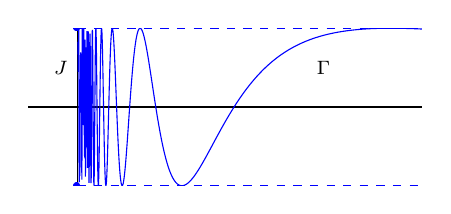
\begin{tikzpicture}
        \begin{axis}[
            axis lines* = middle,
            height=2cm,
            width=5cm,
            scale only axis=true,
            ytick=\empty,
            xtick=\empty,
            xmin=-0.1,
            xmax=0.7,
            ymin=-1,
            ymax=1,
        ]
        \addplot[
            domain=0.001:0.8,
            samples=1000,
            color=blue,
            smooth,
        ]
        {sin(deg(1/x))};
        \draw[blue, dashed] (0,1) -- (1,1);
        \draw[blue, dashed] (0,-1) -- (1,-1);
        \node at (0,0.5) [left] {\scriptsize $J$};
        \node[blue] at (0,1) {\tiny \textbullet};
        \node[blue] at (0,-1) {\tiny \textbullet};

        \node at (0.5, 0.5) {\scriptsize $\Gamma$};
        \end{axis}
        \end{tikzpicture}
        \caption{\textit{Seno del topólogo o de Varsovia.}}
        \label{fig:seno_topologo}
    \end{figure}
\end{enumerate}
\end{ej}

\section{Tabla de comportamiento}%
\label{sec:tabla_de_comportamiento_conx}
En este apartado estudiamos como comporta conexión con respecto a las construcciones del tema \nameref{cha:construcciones}. Se trata de ver cuándo se conserva, cuándo no y qué hipótesis podemos añadir para que se conserve en los casos que no.

\begin{table}[H]
\centering
\begin{tabular}{| c | c | c | c | c |}
\hline
& Subespacios & Cocientes & Productos & Sumas\\
\hline
    Conexión & \ding{55} & \checkmark & \checkmark & \ding{55} \\
    \hline
    Demostración: & $\{0, 1\} \subset \left[ 0, 1 \right]$ & Mantra $2$ & Pivote & Cada sum. es ab. y cerr.\\
    \hline
\end{tabular}
\caption{\textit{Tabla de comportamiento de la conexión con respecto a las construcciones.}}
\end{table}

\begin{prop}
$X \times Y$ conexo $\Leftrightarrow X$ y $Y$ conexo.
\end{prop} 
\begin{demo}
\begin{itemize}
    \item[$\Rightarrow)$] Cada factor es imagen del total a través de la función proyección, que es continua. Como el total es conexo, la imagen continua a través de un conexo es conexa, luego se tiene el resultado.

    \item[$\Leftarrow)$] Fijamos un valor $a \in X$ y entonces vemos que el conjunto
    \[
    Z_y = \underbrace{\left( X \times \{y\} \right)}_{\approx X}\cup \underbrace{\left( \{a\} \times Y \right)}_{\approx Y}
    \]
    es conexo por ser dos conexos que se cortan en el punto $\left( a, y \right)$ (teorema del pivote).
    
    Además, la intersección de todos los $Z_y$
    \[
    \bigcap_{y \in Y} Z_y = \{a\} \times Y \neq \emptyset
    \]
    es no nula, luego por el teorema del pivote de nuevo, tenemos que:
    \[
    \bigcup_{y \in Y} Z_y = X \times Y \text{ conx.}
    \]
    \begin{figure}[H]
        \centering
        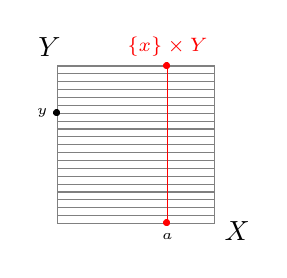
\begin{tikzpicture}
            \draw[gray] (0,0) rectangle (2,2);
            \foreach \y in {0.1, 0.2, ..., 2}
                {
                    \draw[gray,-] (0,\y) -- (2,\y);
                }
            \node at (0,1.4) {\tiny\textbullet};
            \node at (0,1.4) [left] {\tiny $y$};

            \node[red] at (1.4,0) {\tiny\textbullet};
            \node at (1.4,0) [below] {\tiny $a$};

            \draw[red,-] (1.4,0) -- (1.4,2);
            \node[red] at (1.4,2) {\tiny\textbullet};
            \node[red] at (1.4,2) [above] {\scriptsize $\left\{ x \right\} \times Y$};

            \node at (-0.1,2) [above] {$Y$};
            \node at (2,-0.1) [right] {$X$};
        \end{tikzpicture}
        \caption{\textit{Representación de que el producto conexos es conexo: cada línea del cuadrado es un $X \times \left\{ y \right\}.$}}
    \end{figure}
\end{itemize}
\end{demo}


\chapter{Componentes conexas y\texorpdfstring{\\}{} conexión local}%
\label{cha:componentes_conexas_y_conexion_local}
Una vez estudiada la noción de conexión, vamos a repetir el procedimiento que venimos haciendo varios capítulos atrás y vamos a estudiar la versión local de la propiedad. Además, es de especial interés estudiar unos subespacios especiales en cuanto a conexión se refiere que son las componentes conexas y que permiten dividir el espacio en una partición de conjuntos conexos.

\section{Componentes}%
\label{sec:componentes}
Cuando un conjunto no es conexo, tiene sentido preguntarse en cada punto ¿cuál será el mayor subespacio que contiene al punto y que sí es conexo? Porque trabajar en dicho subespacio cuando estemos trabajando en entornos del punto permitirá trabajar como si de un conexo se tratara. Además, este mismo subespacio será el mayor conexo que contiene también a otros puntos distintos, luego en cierta manera podemos verlo como una ``clase de equivalencia'' que asocia puntos con el mismo subespacio conexo maximal.

\begin{defi}[Componente Conexa]
Sea $X$ un espacio topológico, definimos una \textbf{componente conexa} de dicho espacio como un subespacio conexo maximal.
\end{defi}

Aunque la definición anterior es correcta y va en la línea de la intuición explicada al comienzo de la sección, necesitamos formalizar de alguna forma como se calculan dichas componentes conexas cuando nos dan un punto concreto. Esto nos va a permitir no sólo calcular la componente conexa a la que pertenece un punto, sino caracterizar las propiedades que éstas pueden tener dentro del espacio topológico.

\begin{prop}[Caracterización de componentes conexas]
Sea $X$ un espacio topológico y $a\in X$ un punto del mismo, el conjunto:
\[
C(a) := \bigcup_{C \ni a} C \mbox{ donde }C \mbox{ es conexo}
\]
verifica las siguientes propiedades:
\begin{itemize}
\item Es conexo
\item Para cualquier $E\subset X$ conexo tal que $C(a) \cap E \neq \emptyset$, se cumple que $E \subset C(a)$.
\end{itemize}
por tanto, podemos decir que $C(a)$ es la componente\footnote{Puesto que si verifica las dos propiedades mencionadas, entonces es un subespacio conexo maximal.} conexa a la que pertenece $a$.
\end{prop}
\begin{demo}
En primer lugar, como la intersección de todos los conexos de la unión es no vacía (porque $a$ está contenido en la misma) y todos son conexos, por el teorema del pivote el conjunto $C(a)$ es conexo.

Por otro lado, si escogemos un conexo $E\subset X$ tal que $C(a) \cap E \neq \emptyset$, por el teorema del pivote, el conjunto $W := C(a)\cup E$ es conexo y contiene a $a$. Precisamente por esto último, este conjunto es uno de los de la unión que definía $C(a)$, luego $W \subset C(a) \Rightarrow E\subset E \cup C(a) \subset C(a)$, es decir, $E\subset C(a)$.
\end{demo}

\begin{obs}
Tras la caracterización anterior, hay un par de observaciones que son evidentes:
\begin{itemize}
\item Las componentes conexas de dos puntos distintos $a \neq b$ son la misma o son disjuntas, pues si la intersección es no vacía la una está contenida en la otra y viceversa, es decir, son la misma.
\item Como se trata de un conjunto conexo, sabemos que la adherencia $\overline{C(a)}$ es un conjunto conexo. Sin embargo, como $\overline{C(a)}$ es un conjunto conexo que contiene a $a$, tiene que estar contenido en $C(a)$, luego $\overline{C(a)} \subset C(a) \Rightarrow C(a) = \overline{C(a)}$.
\end{itemize}
Las dos observaciones anteriores sumadas a la caracterización, permiten darse cuenta de que el espacio $X$ se puede escribir como unión disjunta
\[
X = \bigsqcup_{C\subset X} C \mbox{ donde }C \mbox{ es comp. conexa}
\]
es decir, que $X$ es una partición de cerrados conexos y disjuntos.
\end{obs}

\begin{ej}
\begin{enumerate}
    \item $X_{\text{discreto}}: C\left( x \right) = \{x\}$ (puntos abiertos y cerrados)
    \item $\mathbb{Q}_u : C\left( p \right) = \{p\}$ (todo intervalo de $\mathbb{R}$ tiene racionales)
    \item $\left( \mathbb{R}, \mathcal{T}_{[, )} \right): C\left( t \right) = \{t\}$ ($\mathbb{R} = \left( \leftarrow, a \right) \cup \left[ a, \rightarrow \right)$ abierto y cerrado)
    \item $X = \{0, Y_k,\ k \ge 1\} : \begin{cases}
        C\left( 0 \right) = \{0\} \text{ cerrado, no abierto} \left( \{\frac{1}{k}: k\ge 1 \}  \text{ no cerr.}\right)\\
        C\left( \frac{1}{k} \right) = \{\frac{1}{k}\} \text{ cerrado y abierto.} 
    \end{cases} $
\end{enumerate}
\end{ej}

\begin{defi}[Espacio totalmente disconexo]
Sea $X$ un espacio topológico, decimos que es \textbf{totalmente disconexo} si y sólo si $\forall a \in X : C(a) = \{a\}$ o, lo que es lo mismo, las componentes conexas del conjunto son los puntos.
\end{defi}

\begin{prop}
Sean $X$ e $Y$ espacios topológicos y $X\times Y$ el espacio topológico producto, las componentes conexas de $X \times Y$ son los productos de componentes conexas de $X$ y de $Y$.
\end{prop}
\begin{demo}
\begin{itemize}
\item $\Rightarrow $ Las componentes conexas del producto son producto de componentes conexas.

Sea $C \subset X \times Y$ una componente conexa del producto, si denotamos por $p$ y $q$ a las proyecciones sobre cada factor, entonces $p\left( C \right)$ y $q\left( C \right)$ son conexos en $X$ e $Y$ respectivamente (por ser imagen continua de conexo). Estos conexos estarán a su vez contenidos en alguna componente conexa del factor de forma que:
\[
\begin{cases}
    p\left( C \right) \subset E \stackrel{\text{c.c}}{\subset}  X\\
    q\left( C \right) \subset F \stackrel{\text{c.c}}{\subset}  Y
\end{cases} \Rightarrow C \subset E \times F \mbox{ donde } E \times F \mbox{ es conexo}
\]
y como $C$ es un subespacio conexo maximal, necesariamente debe ocurrir que $C = E\times F$.

\item $\Leftarrow$ El producto de componentes conexas es una componente conexa

Supongamos que tenemos dos componentes conexas $C_x$ y $C_y$ de $X$ e $Y$ respectivamente y que $\exists E \subset X$ conexo tal que $E\cap C_x \times C_y \neq \emptyset$, pero $E \not\subset C$. Como $E\cap C_x \times C_y \neq \emptyset$, por el teorema del pivote, $E\cup C_x \times C_y$ es conexo. La proyección $p(E\cup C_x \times C_y)$ es el conjunto conexo formado por los valores $x\in X : x\in E_x \ \vee \ x\in C_x$ y como $C_x \subset p(E\cup C_x \times C_y)$ y es conexo maximal, sabemos que $C_x = p(E\cup C_x \times C_y)$. Un razonamiento análogo para $q$ revela que $C_y = q(E\cup C_x\times C_y)$. Por tanto, hemos conseguido que $E\cup C_x\times C_y = C_x \times C_y$, es decir, que $E\subset C_x \times C_y$, luego absurdo.
\end{itemize}
\end{demo}

\section{Conexión local}%
\label{sec:conexion_local}
En ocasiones es muy útil poder tener la certeza de que puedo trabajar en cada punto de forma local sabiendo que se cumple cierta propiedad. Para ello, vamos a definir qué significa ser conexo localmente y cómo puede esta definición ayudar a satisfacer la cuestión mencionada.

\begin{defi}[Localmente Conexo]
Sea $X$ un espacio topológico, decimos que es \textbf{localmente conexo} si y sólo si para todo punto $x \in X$ existe una base de entornos $\mathcal{B}^x$ formada por entornos abiertos conexos.
\end{defi}

\begin{prop}[Caracterización de conexión local]
Sea $X$ un espacio topológico, este es localmente conexo si y sólo si las componentes conexas de un abierto son abiertas.
\end{prop}
\begin{demo}
\begin{itemize}
    \item[$\Rightarrow)$] 
    
	Vamos a ver que las componentes conexas son entornos de todos sus puntos. Para ello, consideremos $x \in C \stackrel{\text{c.c}}{\subset} U \ab X$. Como $X$ es localmente conexo, con seguridad existirá un $U^x \ab X$ conexo y contenido en $U$ (porque como hay una base de entornos de abiertos conexos, $U$ debe contener alguno). La conexión de $U^x$ implica que $U^x \subset C$ por ser esta componente conexa, luego acabamos de demostrar que $C$ es entorno de todos sus puntos, es decir, abierto. 
	
    \item[$\Leftarrow)$]
    
    Dado un punto $x\in X$, basta con que escojamos como base de entornos las componentes conexas de los abiertos que contienen al punto
    \[
    \mathcal{B}^x := \{C\left( x \right) \stackrel{\text{c.c}}{\subset} U \ab X : x \in U\}			\]
    Dicho conjunto es base de entornos porque cada $C(x)$ es entorno (por ser abierta) y cualquier otro entorno debe contener a alguna, puesto que por ser entorno contendrá algún abierto que contenga al punto y, en consecuencia, alguna de las componentes conexas del conjunto.
\end{itemize}
\end{demo}

\begin{obs}
Sin muchísima dificultad, es sencillo demostrar que la definición de conexión local puede prescindir de la apertura de los conexos que forman la base de entornos, esto es, que la definición dada es equivalente a: ``$X$ es localmente conexo si y sólo si $\forall x \in X,\ \exists \mathcal{V}^x$ base de entornos conexos''.
\end{obs}

\begin{ej}[Esencial]
$\{0, \frac{1}{k} : k \ge 1\} = Y \subset \mathbb{R}_u$ \underline{no} es localmente conexo. 
\begin{demo}
    La $\text{c.c}\left( 0 \right) = \{0\}$ no es abierto. Directamente:
    \begin{align*}
        0 \in \underbrace{V}_{\text{ent. de } 0 \in \mathbb{R}} \cap Y &\Rightarrow V \supset \left( 0, \varepsilon \right),\ \exists 0 < \underbrace{\theta}_{\not\in \mathbb{Q}} < \frac{1}{k} < \varepsilon < 1\\
        &\Rightarrow V\cap Y \subset \underbrace{\left( \leftarrow, \theta \right)}_{\ni 0} \cup \underbrace{\left( \theta, \rightarrow \right)}_{\ni \frac{1}{k}}  \Rightarrow V \cap Y \text{ no conexo.} 
    .\end{align*}
\end{demo}
\end{ej}

\begin{ej}
Supongamos que tenemos un conjunto de segmentos verticales que convergen al segmento de la izquierda del todo, que también incluimos en el conjunto, tal y como muestra la figura
    \begin{figure}[H]
        \centering
        \begin{tikzpicture}
            \foreach \x in {0, 0.005, 0.01, 0.02, 0.035, 0.1, 0.25, 0.5, 0.8, 1.5, 3, 6}
                \draw[-, gray] (\x, 0) -- (\x, 2);
        \end{tikzpicture}
        \caption{\textit{Ejemplo}}
    \end{figure}
¿Es este conjunto localmente conexo? La respuesta es no. Para ver esto, tenemos que ver que para cada punto existe una base de entornos formada por abiertos conexos. En cualquier segmento que no sea el de la izquierda del todo, podemos encontrar una bola $B(x,\rho)$ con $\mathbb{\rho}$ real tal que dicha bola no interseque con ningún otro segmento del conjunto, luego la colección $\{B(x,\varepsilon) : 0 < \varepsilon < \rho\}$ es una base de entornos de cualquier punto de estos segmentos. El problema principal está en el segmento de la izquierda del todo, pues cualquier bola $B(x,\rho)$ centrada en dichos puntos necesariamente interseca con muchos otros segmentos (porque los segmentos convergen hacia la izquierda). Con esto hemos demostrado que cualquier entorno de uno de estos puntos, necesariamente contiene puntos de otros segmentos y entonces el entorno inicial siempre será disjunto.
\end{ej}

\section{Tabla de comportamiento}%
\label{sec:tabla_de_comportamiento_loc_conx}
En este apartado estudiamos como se comportan la conexión local con respecto a las construcciones del tema \nameref{cha:construcciones} para ver cuándo se conservan, cuándo se pierden y qué podemos añadir para no perderlas.

%TODO: Fix tabla. En subespacios los abiertos sí heredan
\begin{table}[H]
\begin{tabular}{| c | c | c | c | c |}
\hline
& Subespacios & Cocientes & Productos & Sumas\\
\hline
Conexión local & \begin{tabular}{cc} \ding{55} & $\checkmark_{abierto}$ \end{tabular} & \checkmark & \begin{tabular}{cc} \checkmark & \checkmark \end{tabular} & \begin{tabular}{cc} \checkmark & \checkmark \end{tabular} \\
\hline
Demostración: & Ejemplo esencial & No banal & Prod. ent. conx. & Suma como sum's\\
\hline
\end{tabular}
\caption{\textit{La tabla nos indica como se conserva la compacidad local en las construcciones que hemos visto. Las sumas y los productos son finitos.}}
\end{table}


\begin{prop}
Sea $X$ un espacio topológico localmente conexo y $f : X \rightarrow Y$ una identificación a un espacio $Y$, el espacio $Y$ es localmente conexo.
\end{prop}
\begin{demo}
Para demostrar la local conexión, vamos a demostrar que las componentes conexas de abiertos son abiertas. Para ello, tomemos un abierto $V\ab Y$ y una componente conexa suya $C \subset V$ y veamos que tiene que ser abierta.

\begin{center}
        \includegraphics[scale=0.3]{images/dem_loc_conx_loc_conx} 
\end{center}

En primer lugar, por la continuidad de $f$, $f^{-1} V \ab X$ así que la local conexión de $X$ nos asegura que $\exists U^x \ab f^{-1}V$ pero además este es conexo. Como $f$ es continua, $f(U^x)$ es conexo y contiene a $x$, luego por la maximalidad de $C$ debe ocurrir que $f(U^x)\subset C$. Por tanto, ahora vemos con facilidad que $f^{-1} C \subset f^{-1}V$ contiene a $U^x$, es decir, hemos visto que la preimagen $f^{-1}C$ es abierta en $X$ y como es abierto saturado $C$ es abierto.
\end{demo}
